\documentclass{article}
\usepackage{graphicx}
\usepackage{minted}
\usepackage{xcolor}
\usepackage[romanian]{babel}

\title{Transformata Fourier - Ghid vizual}
\author{Andra Alexandrescu}
\date{Proiect în cadrul cursului de Mecanică - Noiembrie 2025}

\begin{document}

\maketitle

\section*{Introducere}
\paragraph{}Înainte de a vorbi de transformata Fourier care face obiectul discuției și al proiectului, vom descrie ca început conceptul analizei Fourier.
\section*{Analiza Fourier}
\paragraph{În cadrul analizei Fourier, a fost demonstrat că orice semnal periodic poate fi scris ca o sumă infinită de funcții trigonometrice (funcții cosinus și sinus).}

\paragraph{}Pentru exactitate, orice funcție, \(f(t)\), definită pe intervalul \(t \in (0,\pi)\), poate fi exprimată ca o combinație liniară infinită de sinusoide, \(f(t) = a_1\sin(t)+a_2\sin(2t)+a_3\sin(3t)+\ldots\) și că valoarea coeficienților \(a_n\) poate fi calculată ca aria de sub curba \(f(t) \sin(nt)\), care este dată de formula \(a_n = \frac{2}{\pi} \int_{0}^{\pi} f(t)\sin(n t)\, dt\).

\paragraph{} Ca aplicație am decis asupra demonstrării modalității de identificare a parametrilor unui semnal original, cu scopul de a-l reconstrui folosind serii Fourier și de a ilustra principiile fundamentale definite anterior. 

\subsection*{ Determinarea coeficiențiilor ca aria de sub curba \(f(t) \sin(nt)\) }
    \textbf{Scop}: \textbf{Demonstrarea limitelor practice} ale metodei
    \paragraph{} Am ales câteva funcții drept studiu de caz, urmărind a observa comportamentul raportat la funcții pare, funcții exponențiale netede, funcții cu dicontinuități și funcții pentru care seriile Fourier clasice sunt incompatibile.
\begin{minted}{python}
n_max = 50
functii = [
    ("f(t) = cos(3t)", lambda t: np.cos(3*t)),
    ("f(t) = e^(-t)", lambda t: np.exp(-t)),
    ("f(t) = semn(t-np.pi/2)", lambda t: np.where(t<np.pi/2, 1, -1)), 
    # centrat la np.pi/2
    ("f(t) = 3*sin(2*np.pi*5*t))", lambda t: 3*np.sin(2*np.pi*5*t))
]

# afisarea convergentei Fourier
t = np.linspace(0.01, np.pi-0.01, 1000) # returneaza 1000 de sample-uri
# egale ca si distanta in intervalul 0.01 si np.pi-0.01,
# ca sa evite capetele

L_coeficienti_functii = [] # se calculeaza coef Fourier pt fiecare functie
for str_formula, f in functii:
    L_coeficienti = []
    for n in range(1, n_max+1):        
        # integram produsul intre functia curenta 
        # si sin(n*t) pe intervalul 0, np.pi
        integrala, _ = integrate.quad(lambda t: f(t)*np.sin(n*t), 0, np.pi) 
        # functia quad primeste (f, a, b) adica il 
        # integreaza pe f de la a la b 
        # (stiind neaparat ca integrala converge)
        a_n = (2/np.pi)*integrala
        L_coeficienti.append(a_n)
    L_coeficienti_functii.append((str_formula, f, L_coeficienti))
    # lista de tupluri de forma string formula, 
    # f lista de coef a1... an_max
    
# afis functii impreuna cu coef Fourier coresp

# afisare coef Fourier
fig, axs = plt.subplots(len(functii), 2, figsize=(15, 10))
axs = axs.flatten()

for i, (str_formula, f, coeficienti) in enumerate(L_coeficienti_functii):
    ax_stg, ax_dr = axs[2*i], axs[2*i+1]
    ax_stg.plot(t, f(t))
    ax_stg.set_title(f'functia: {str_formula}')
    ax_stg.set_xlabel('t')
    ax_stg.set_ylabel('f(t)')
    ax_stg.grid(True)

    n_valori = range(1, len(coeficienti)+1)
    ax_dr.stem(n_valori, coeficienti)
    ax_dr.set_title(f'coeficientii Fourier: {str_formula}')
    ax_dr.set_xlabel('n')
    ax_dr.set_ylabel('an')
    ax_dr.set_xticks(range(0, n_max+1, 10))
    ax_dr.grid(True)

plt.tight_layout()
plt.savefig(fname="fig1.pdf", format="pdf")
plt.show()
\end{minted}

\begin{figure}[H]
    \centering
    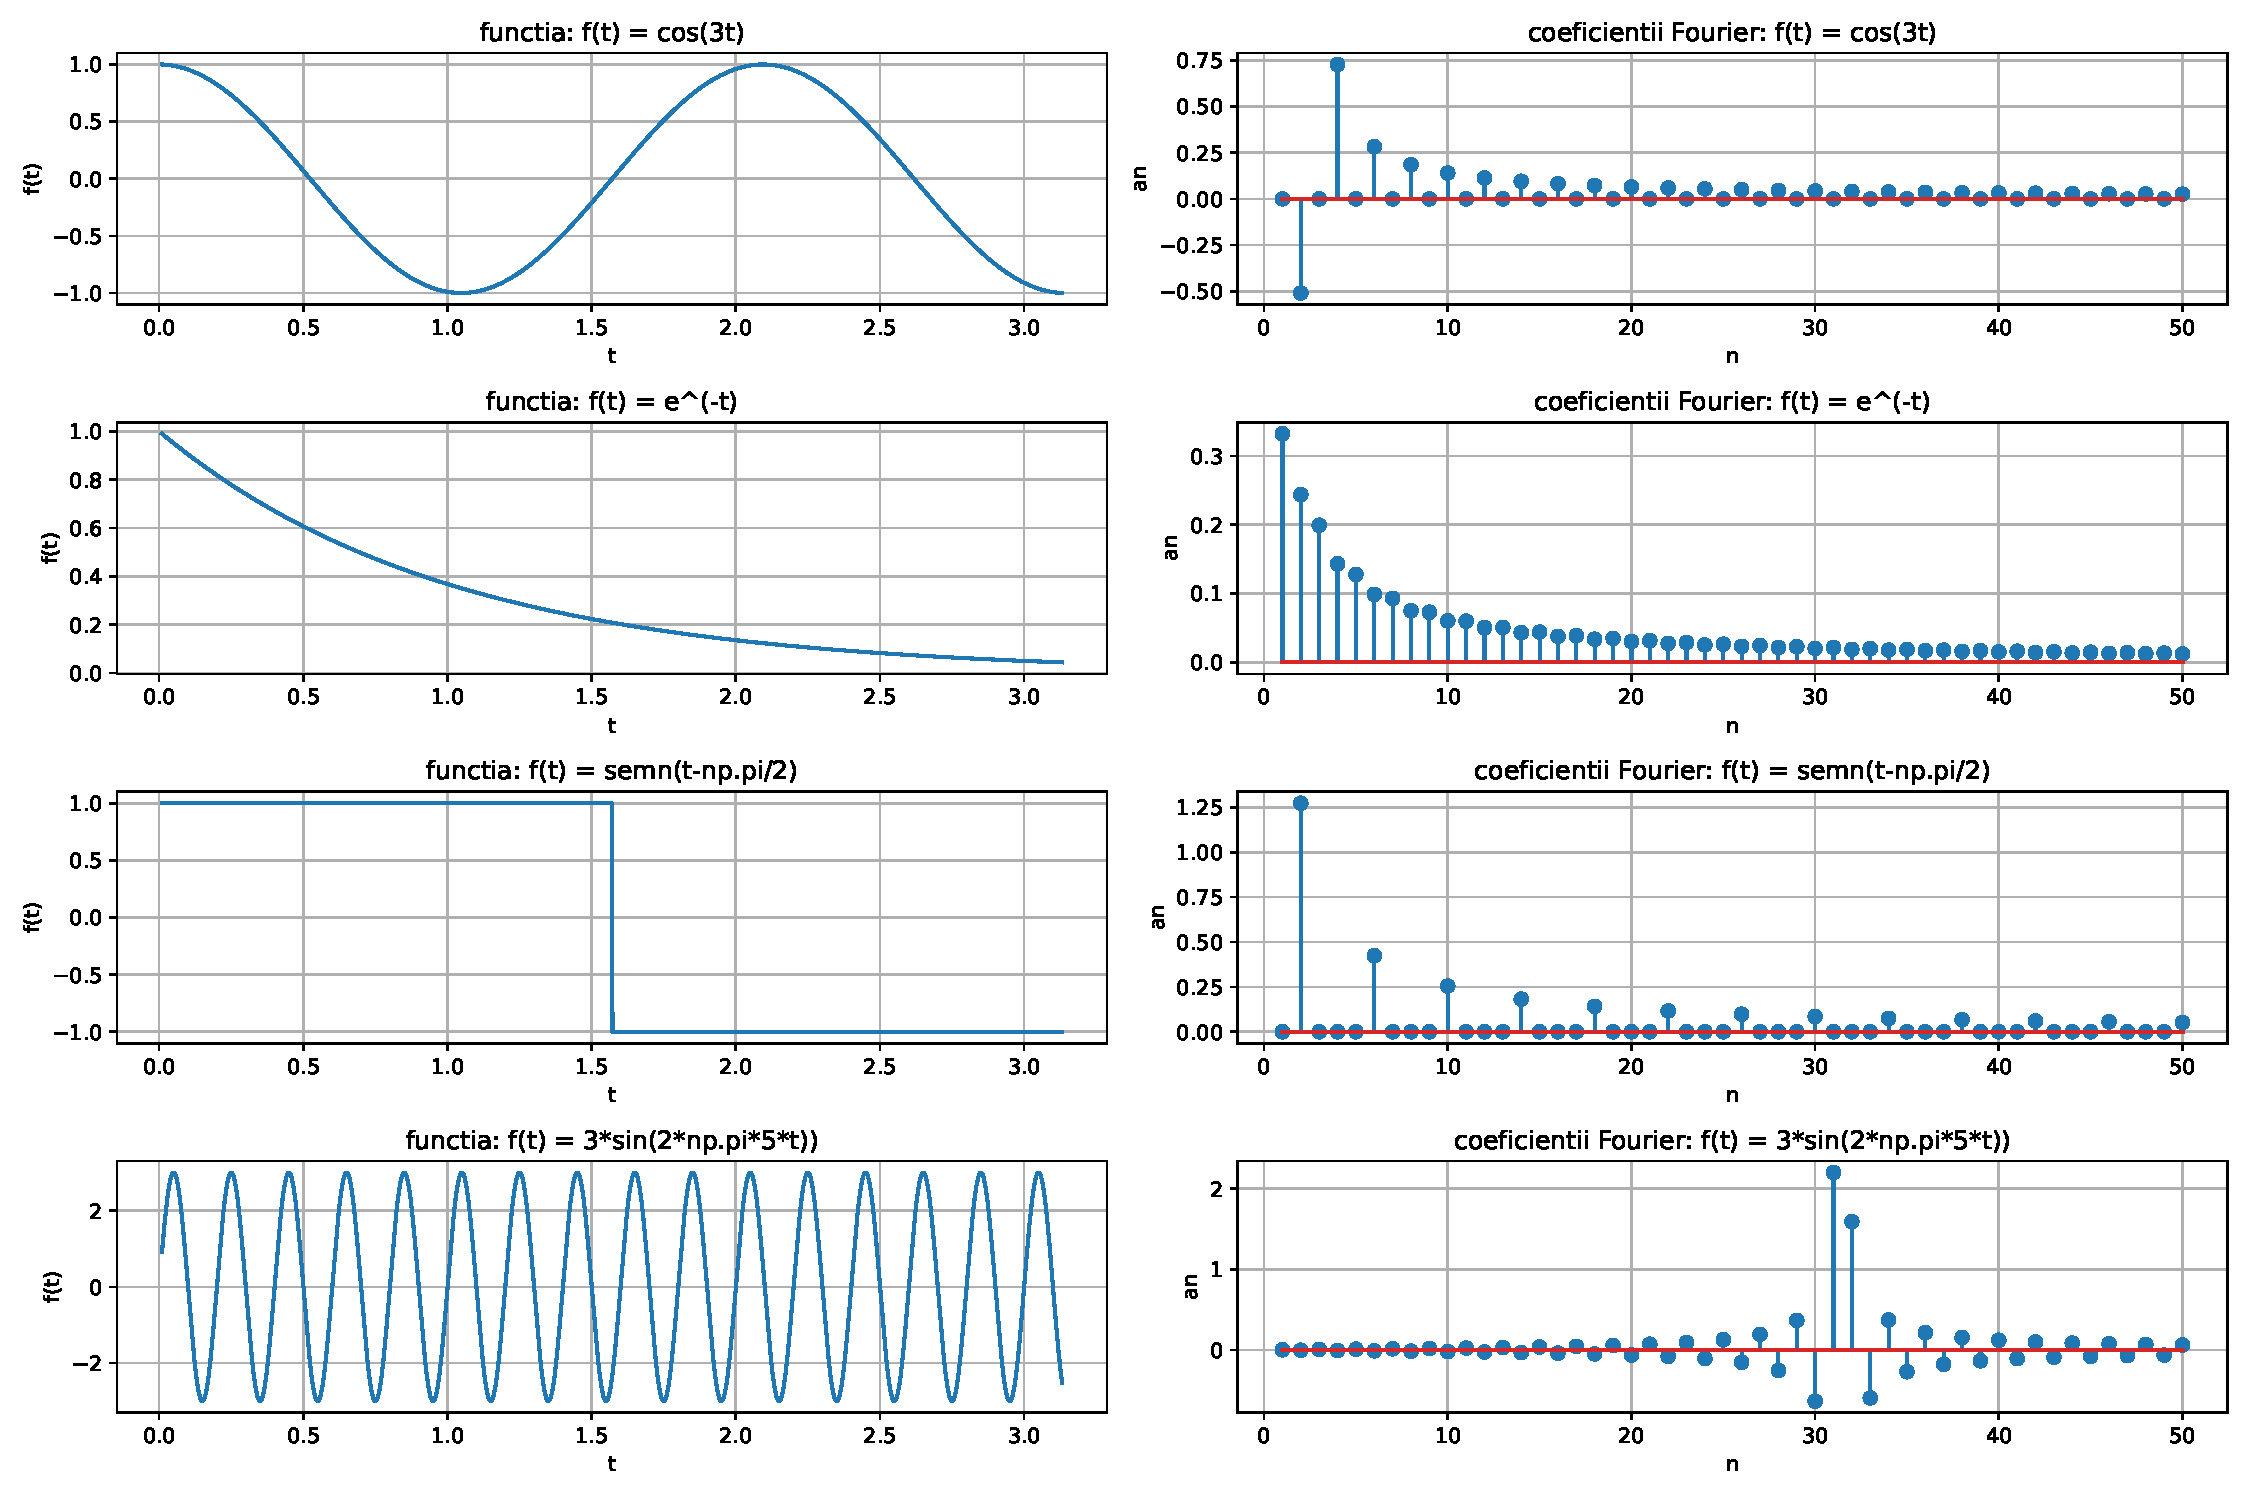
\includegraphics[width=0.7\textwidth]{fig1.pdf}
    \caption{Funcțiile și coeficienții asociați acestora}
    \label{fig:fig1}
\end{figure}

\begin{minted}{python}
fig, axs = plt.subplots(len(functii), 2, figsize=(15, 4*len(functii)))

for i, (str_formula, f, coeficienti) in enumerate(L_coeficienti_functii):
    ax_stg, ax_dr = axs[i, 0], axs[i, 1]
    y_original = f(t)
    ax_stg.plot(t, y_original, 'k-', linewidth=2, label='functie originala')
    
    n_termeni = [5, 10, 20, 50]
    # demonstrare de cum converge seria Fourier
    # pe masura ce se adauga mai multi termeni in suma
    culori = plt.cm.tab10(np.linspace(0, 1, len(n_termeni)))

    for j, termen in enumerate(n_termeni):
        y_fourier = 0
        for n in range(min(termen, len(coeficienti))):
            y_fourier += coeficienti[n]*np.sin((n+1)*t) # an*np.sin(an*t)

        ax_stg.plot(t, y_fourier, '--', color=culori[j], label=f'Fourier (nr termeni = {termen})')
    
    ax_stg.set_xlabel('t')
    ax_stg.set_ylabel('f(t)')
    ax_stg.set_title(f'aprox fourier: {str_formula}')
    ax_stg.set_xlim(0, np.pi)
    ax_stg.legend()
    
    y_fourier_complet = 0
    for n in range(min(n_max, len(coeficienti))):
        y_fourier_complet += coeficienti[n]*np.sin((n+1)*t) # an*np.sin(an*t)

    eroare = np.abs(y_original-y_fourier_complet) # modulul dif e eroarea
    
    ax_dr.plot(t, eroare, 'r-', linewidth=1)
    ax_dr.set_xlabel('t')
    ax_dr.set_ylabel('eroare absoluta')
    ax_dr.set_title(f'eroarea de aproximare: {str_formula}')
    ax_dr.set_xlim(0, np.pi)

plt.tight_layout()
plt.show()

\end{minted}

\begin{figure}[H]
    \centering
    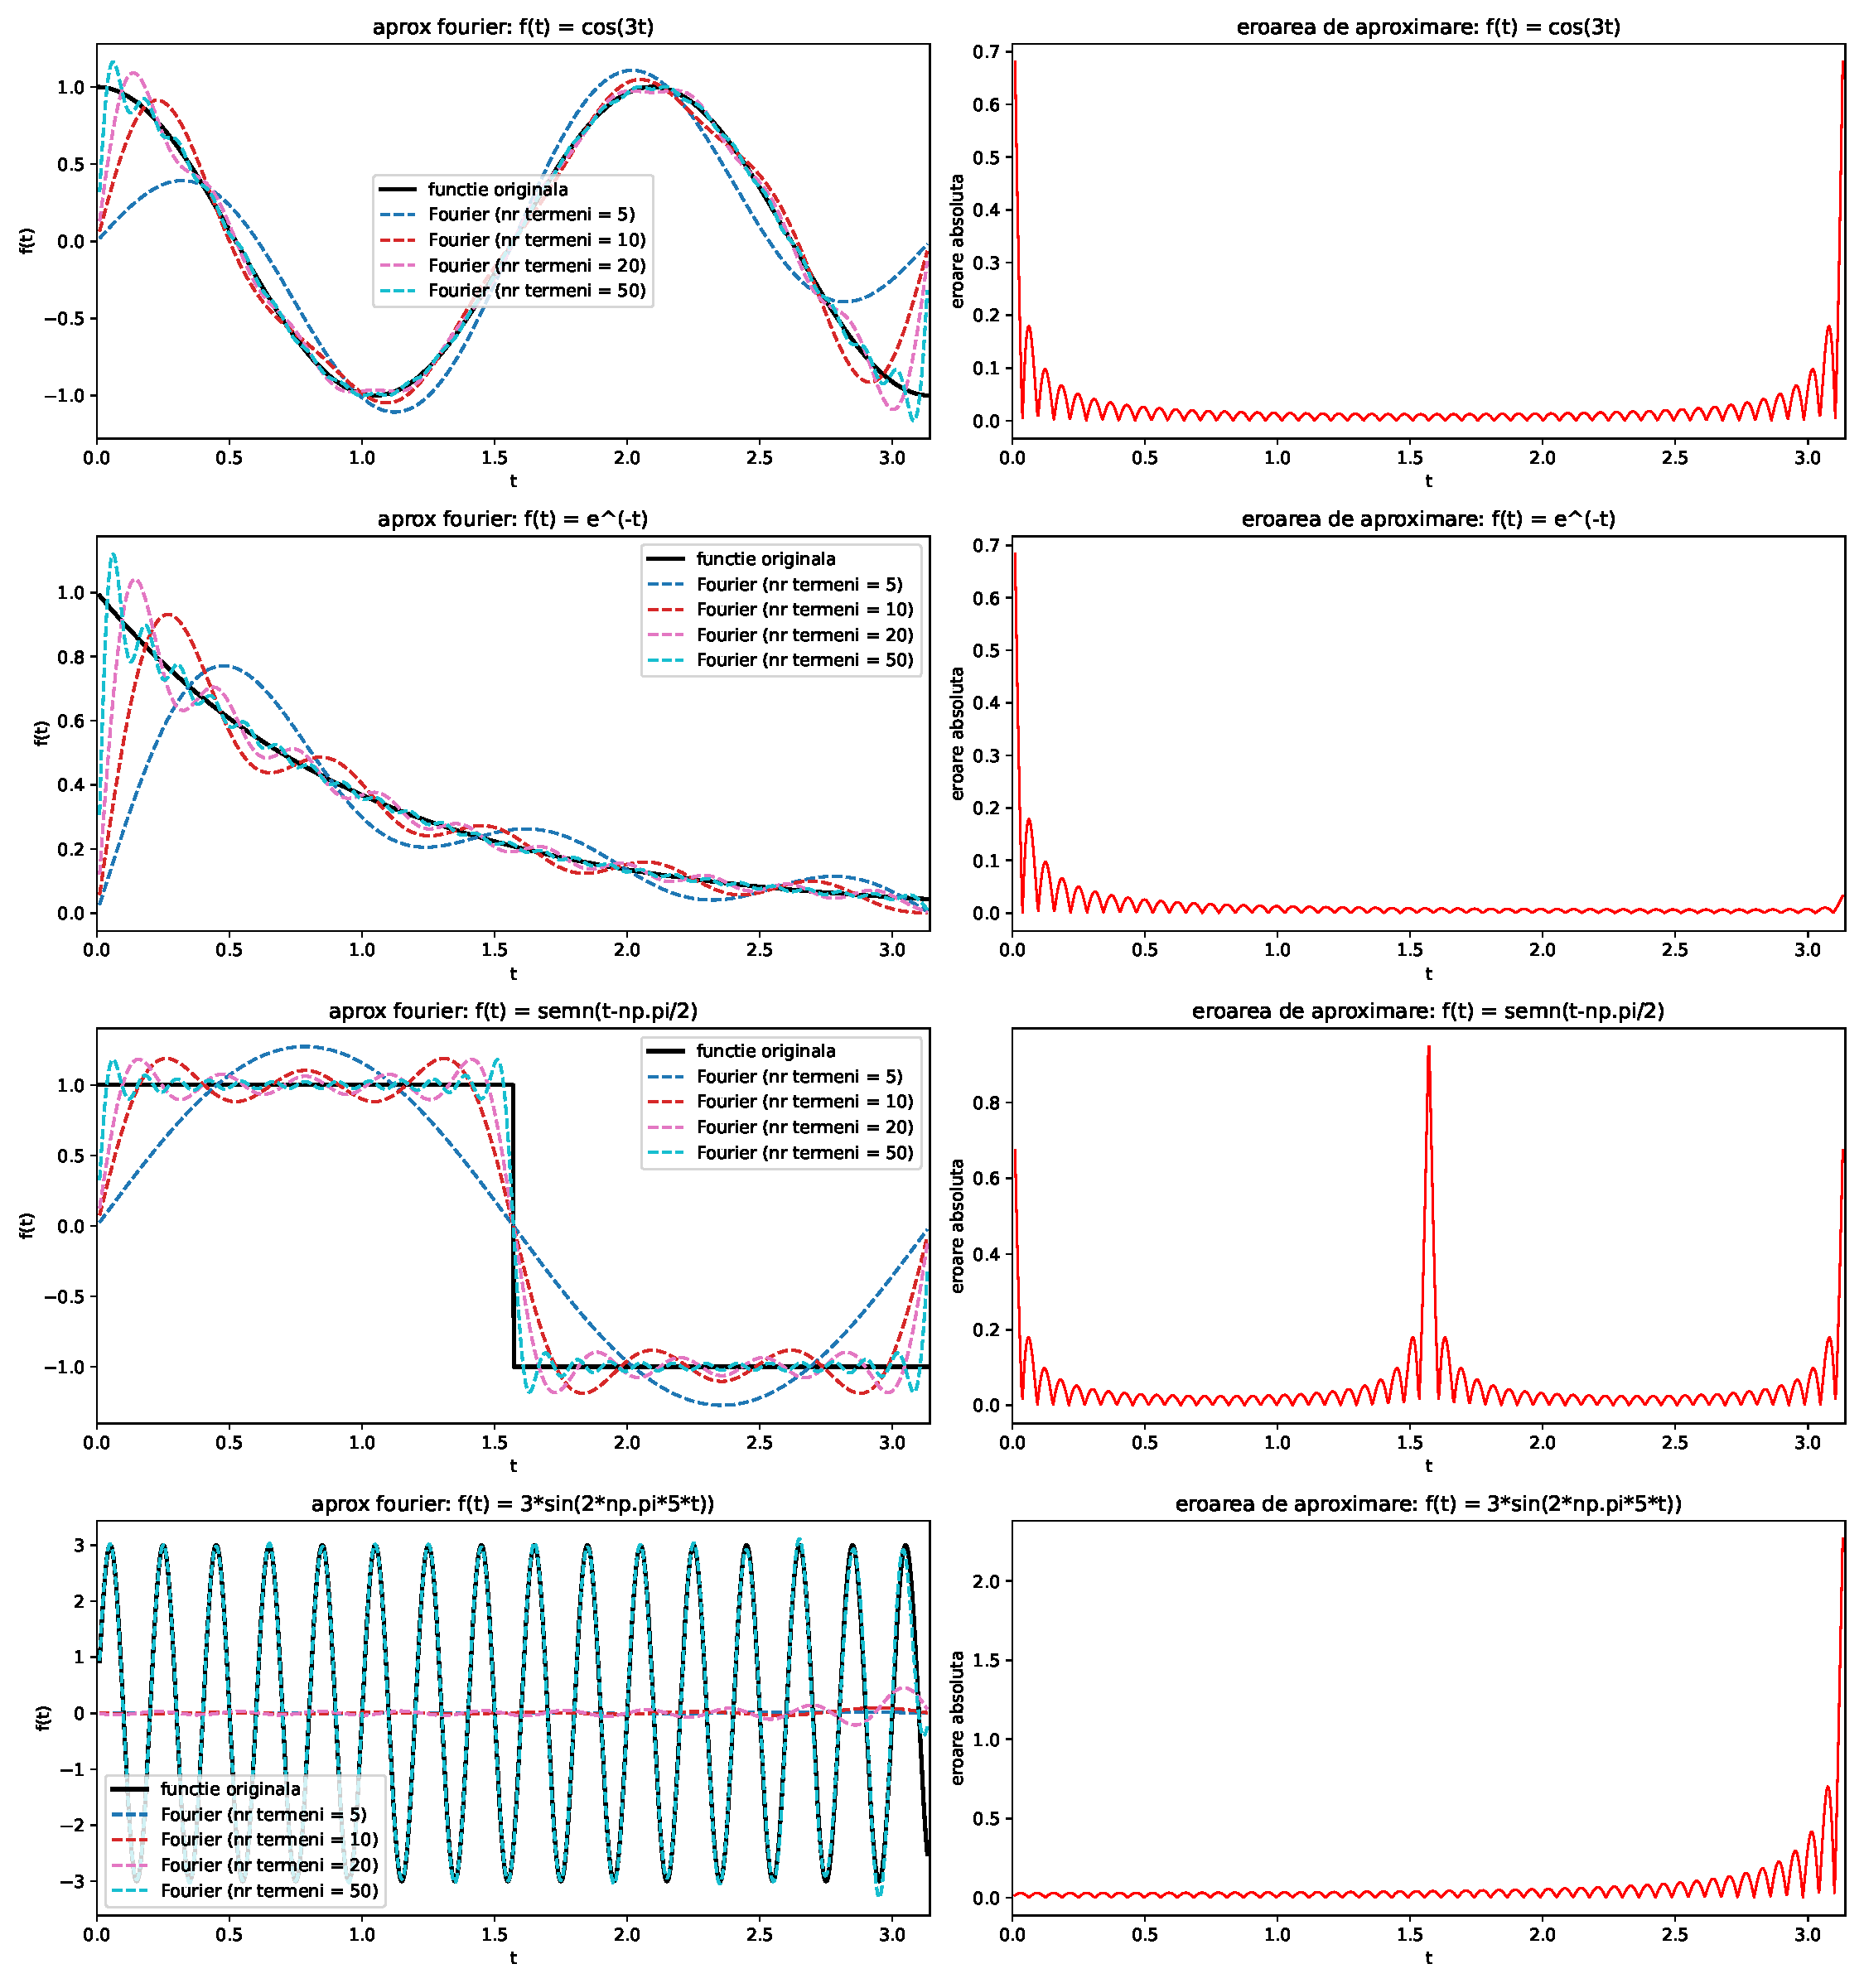
\includegraphics[width=0.7\textwidth]{fig2.pdf}
    \caption{Convergența Fourier și eroarea absolută}
    \label{fig:fig2}
\end{figure}

\begin{itemize}
    \subsection*{Observații:}
    \item \textbf{Calcul coeficienți Fourier}: Fiecare coeficient $a_n$ indică cât de mult din componenta $\sin(n\cdot t)$ este prezentă în funcția dată.
    \item \textbf{Reconstrucție prin sume parțiale}: Arată cum adăugarea de termeni îmbunătățește aproximarea.

    \subsection*{Proprietăți caracteristice fiecărui studiu de caz:}
    \item pentru \(\cos(3t)\) se observă cum seriile Fourier sinusoidale (funcții impare) aproximează funcții pare
    \item pentru \(e^{-t}\) arată o convergență rapidă, fiind o funcție netedă dar neperiodică
    \item pentru \(semn(t-\pi/2)\) determină ideea de însumare a multor oscilații cu scopul de a se anula reciproc în vecinătatea discontinuității
    \item pentru \(3sin(2\pi5t)\) compunerea de sinusoide eșuează, deoarece încearcă să aproximeze o funcție cu multe oscilații (funcția realizează 31.4 cicluri complete, având o frecvență de 5Hz este echivalentă cu \(10\pi\) radiani)
\end{itemize}

\paragraph{În următorul capitol, vom urmări cum poate ajuta eșantionarea la conversia unui semnal analogic în semnal digital.}

\section*{Discretizarea sau continuitatea unei sinusoide}

\paragraph{Unda sinusoidală în timp continuu:} \(x(t) = A\sin(2\pi ft+\phi)\)

\paragraph{Unda sinusoidală în timp discret:} \(x[n] = A\sin(2\pi fnT+\phi)\) unde \(n\) este indexul eșantionului și \(T\) este perioada de eșantionare.

\paragraph{}Eșantionarea, care e un caz particular de discretizare, transformă un semnal continuu într-un semnal discret, extrăgând valorile instantanee ale semnalului la anumite puncte în timp.

\paragraph{În următoarea secțiune, vom urmări cum poate ajuta eșantionarea la conversia unui semnal analogic în semnal digital.}

\section*{Transformata Fourier}
\begin{itemize}
    \item Transformata Fourier exprimă un semnal dependent de timp ca o sumă continuă, integrată, de unde sinusoidale cu frecvențe care variază pe un interval.
    
    \(X(f) = \int_{-\infty}^{\infty} x(t) e^{-j 2 \pi f t} dt\)
    
    \item Rezultatul transformatei pentru fiecare frecvență indică cât de puternică este acea componentă (amplitudinea) și cum este poziționată în timp (faza, interpretată ca o rotație în planul complex) în cadrul semnalului original. Pentru exactitate, rezultatul transformatei este o funcție, notată de obicei \(X(\omega)\), care oferă informații despre conținutul semnalului original \(x(t)\).
\end{itemize}

\section*{Transformata Fourier discretă}
\paragraph{Transformata Fourier discretă (DFT)} este echivalentul transformatei Fourier continue pentru semnale cunoscute \textbf{doar} în momente separate de timp (eșantioane), adică o secvență finită de date. Așadar, permite analiza semnalelor discrete, spre deosebire de transformata Fourier continuă, care este definită pe semnale continue.

\paragraph{} Un semnal \(x(t)\) care reprezintă o mărime fizică (cum ar fi deformația cauzată de unde gravitaționale, etc.) este eșantionat la intervale regulate, distanțate la \(T\). Notăm \(T\) ca fiind perioada de eșantionare. Astfel, corespunzătoarea frecvență de eșantionare este dată de \(f_s = 1/T\). Timpurile discrete la care eșantionăm semnalul sunt date de:
\(t_n = nT = \frac{n}{f_s} \text{,}  \quad n = 0, 1, 2, \ldots, N-1\)

\paragraph{} Putem considera variabila \(n\) ca fiind un indice întreg care ține evidența timpului și scriem semnalul digital eșantionat cu \(N\) puncte ca \(x[n]\).

\paragraph{} Datorită faptului că semnalul prezintă oscilații, putem introduce ca și concept frecvența unghiulară, având notația de \(\omega_0 = \frac{2 \pi}{N T} \text{,} \quad \omega_m = m \omega_0 = m \frac{2 \pi}{N T}\). Se observă că \(NT\) reprezintă durata totală pentru care semnalul a fost eșantionat. Astfel, frecvența fundamentală \(\omega_0\) corespunde unei unde care completează exact o oscilație pe durata totală de înregistrare. Mai mult, un semnal care oscilează la frecvența \(\omega_m\) va oscila de \(m\) ori în total pe durata înregistrată.

\paragraph{} Concluzionând, transformata Fourier a unui semnal discret se definește ca:
\[
X[m] = \sum_{n=0}^{N-1} x[n] s_m[n] = \sum_{n=0}^{N-1} x[n] e^{-j \frac{2 \pi m n}{N}}
\]
, unde exponențiala complexă este
\[
s_m[n] = e^{-j \omega_m t_n} = ... = e^{-j 2 \pi \frac{m n}{N}}
\]

\paragraph{} Ca aplicație am decis studiul înfășurării semnalului pe cercul unitate și cum \(\omega_m\) generează diverse figuri sau forme de reprezentare animate. 

\subsection*{ Înfășurarea unui semnal sinusoidal pe cercul unitate }

\paragraph{} Formula \(e^{-2\pi j n}\), corespunde unui cerc de rază unitară în planul complex, care este parcurs într-o unitate de timp (\(n = 0, \dots, N-1\)). Adăugând semnalul \(x[n]\), înfășurarea pe cercul unitate de mai sus este "deformată" de amplitudinea semnalului.

\begin{minted}{python}
# timpul e discret, iar pentru a ilustra pe cercul
# unitate punctele consecutive stabilesc o frecv 
# discreta fixata M
frecv = 20
rata_esantionare = 1000
durata = 0.2
T = 1/rata_esantionare # perioada de esantionare
N = durata*rata_esantionare # nr_esantioane
n = np.arange(0, int(N)) # n = 0, 1, ... N-1

tn = n*T # momentele discrete de timp
x_n = 0.7*np.sin(2*np.pi*frecv*tn+np.pi/3)

plt.plot(tn, x_n)
plt.xlabel("t")
plt.ylabel("ampl")
plt.grid(True)
plt.show()

m = np.arange(0, int(N)) # m = 0, 1, ... N-1
omega0 = (2*np.pi)/(N*T) # frecv de infasurare
omegam = m*omega0
#print(omega0, omegam, sep="\n")
M = 1 # frecv discreta fixata pentru a conecta puncte
# discrete consecutive intre ele din cauza faptului
# ca X_discret are dimensiunea NxN
sm_n = np.exp(-1j*omegam[M]*tn)

# ceva f f important, omegam[1] == omega0

#print(sm_n)
X_discret = x_n*sm_n

fig, ax = plt.subplots()
for k in range(len(X_discret)-1): # conecteaza punctele prin
# segmente pe planul complex
    ax.plot([X_discret.real[k], X_discret.real[k+1]],
    [X_discret.imag[k], X_discret.imag[k+1]], color='blue')
ax.scatter(X_discret.real, X_discret.imag, c=np.abs(X_discret), cmap='viridis')
ax.set_xlabel("real")
ax.set_ylabel("imaginar")
ax.grid(True)
ax.set_title("X pe cercul unitate")

k = 35 # indexul esantionului de marcat
xk = X_discret.real[k]
yk = X_discret.imag[k]
ax.scatter([xk], [yk], color='red', marker='x', s=50, zorder=2) # zorder pt suprapunere
ax.plot([0, xk], [0, yk], color='red', linestyle='--', linewidth=0.5)
plt.colorbar(ax.collections[0], label='dist origine')
plt.show()
\end{minted}

\begin{figure}[H]
    \centering
    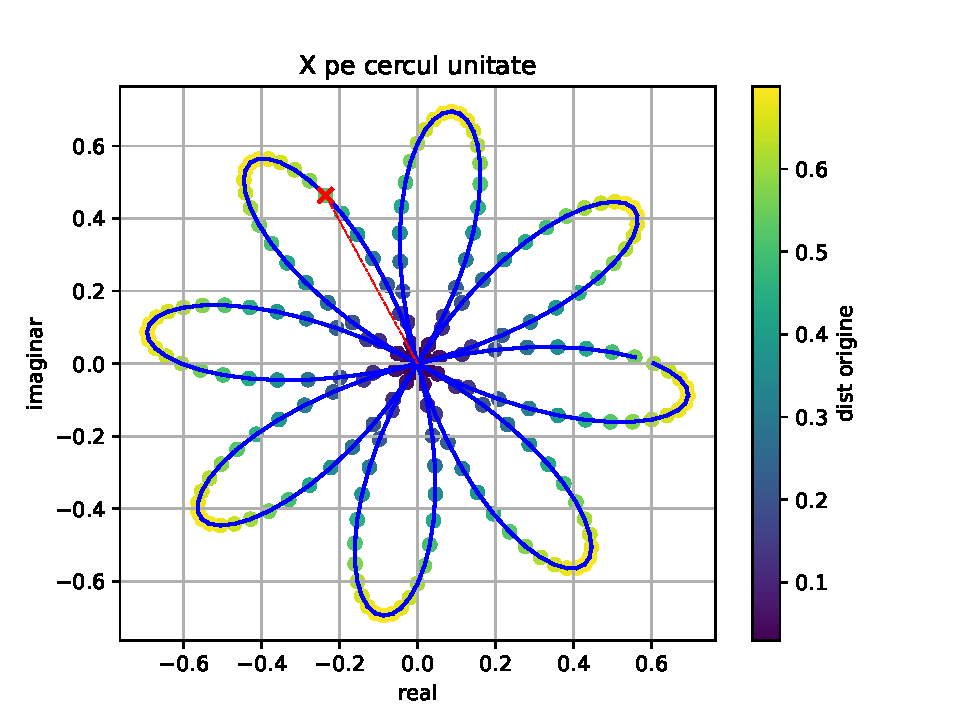
\includegraphics[width=0.7\textwidth]{fig3.pdf}
    \caption{Înfășurarea pe cercul unitate a unei sinusoide pentru M fixat = 1}
    \label{fig:fig3}
\end{figure}

\begin{minted}{python}
fig, axes = plt.subplots(2, 3, figsize=(15, 10)) # 2 linii, 3 coloane
selectie_omegam = np.random.choice(omegam, size=6, replace=False)
axes = axes.flatten()
for i, omega in enumerate(selectie_omegam):
    sm_n = np.exp(-1j*omega*tn)
    X_discret = x_n*sm_n

    ax = axes[i]
    for k in range(len(X_discret)-1):
    # conecteaza punctele prin segmente pe planul complex
        ax.plot([X_discret.real[k], X_discret.real[k+1]], 
        [X_discret.imag[k], X_discret.imag[k+1]], color='blue')
    ax.scatter(X_discret.real, X_discret.imag, c=np.abs(X_discret), cmap='viridis')
    ax.set_xlabel("real")
    ax.set_ylabel("imaginar")
    ax.set_title(f"omega={omega:.2f}")
    ax.grid(True)

plt.tight_layout()
plt.show()
\end{minted}

\begin{figure}[H]
    \centering
    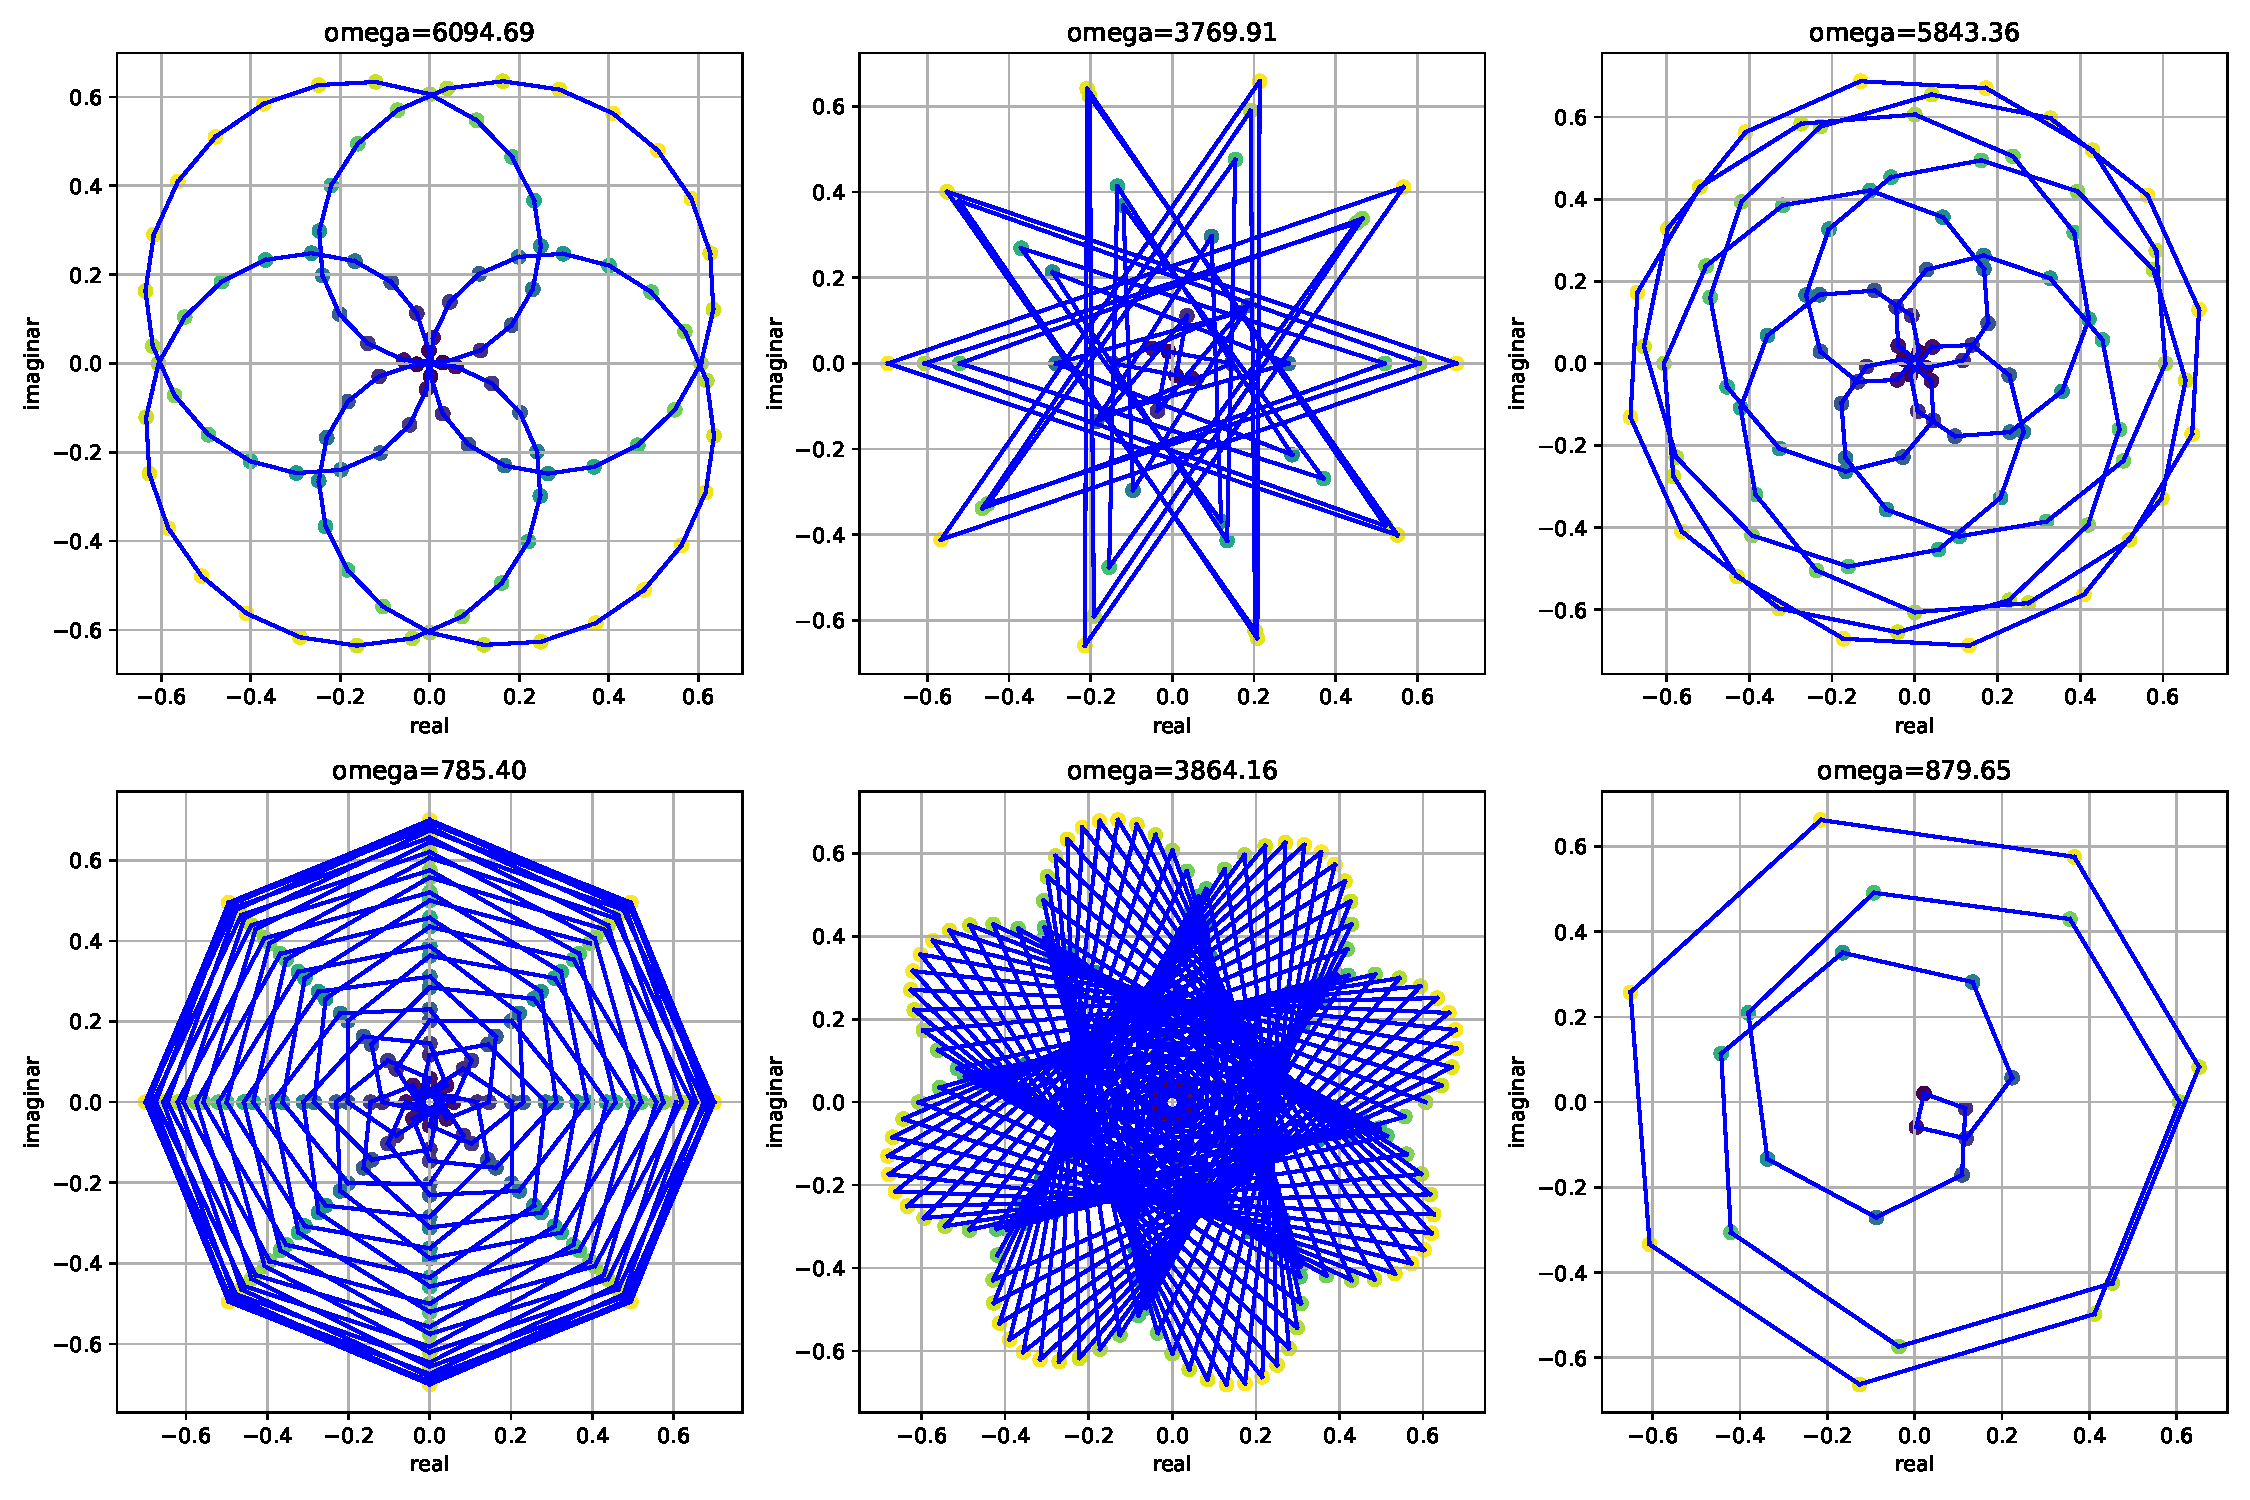
\includegraphics[width=1\textwidth]{fig4.pdf}
    \caption{Înfășurarea pe cercul unitate a unei sinusoide pentru M variabil}
    \label{fig:fig4}
\end{figure}

\begin{itemize}
    \subsection*{Observații:}
    \item \textbf{Frecvențe diferite generează forme distincte}: Fiecare valoare a lui $\omega_m$ produce o figură unică de înfășurare pe planul complex.
    \item \textbf{Densitatea punctelor}: Distribuția punctelor variază semnificativ între diferitele valori ale frecvenței unghiulare.
    \item \textbf{Amplitudini limitate}: Toate punctele se află în intervalul \([-0.6, 0.6]\) pe ambele axe, indicând o amplitudine constantă a semnalului.
    \item \textbf{Faze relative}: Poziția relativă a punctelor indică relațiile de fază dintre diferitele componente de frecvență.

    \subsection*{Proprietăți caracteristice fiecărui studiu de caz:}
    \item pentru \(\omega=3204.42\) se observă că punctele sunt grupate într-o regiune, având faze similare
    \item pentru \(\omega=4461.06\) arată puncte împrăștiate cu faze diverse
\end{itemize}

\paragraph{În plus, cu ajutorul animațiilor asociate acestui proiect, se pot observa apariția punctelor pe fiecare dintre figuri, ordinea punctelor și sensul pe cerc.}

\paragraph{Formele observate pentru diferite valori ale lui \(\omega_m\) demonstrează complexitatea conținutului spectral al semnalului sinusoidal analizat.}

\section*{Matricea Fourier}

Putem folosi o matrice pentru a organiza valorile funcțiilor periodice utilizate în transformata Fourier discretă.

Fie \(\omega = e^{ \left(-\frac{2\pi i}{N}\right)}\), astfel încât
\(e^{\left(-jk\frac{2\pi}{N}\right)} = \omega^{jk}\)


Atunci, putem defini matricea Fourier de dimensiune \(N \times N\):


Putem folosi matricea \(F\) pentru a scrie transformata Fourier discretă în formă matricială:
\[
X = Fx
\]


\( F_{m,k} = \omega^{(m \cdot k)} = e^{-(\frac{2 \pi}{N}) \cdot 1j \cdot m \cdot k} \quad m,k = 0, 1, \dots, N-1, m_{linie}, k_{coloana}\)

\(
F_{m,k} = \omega^{m k}
= e^{-\frac{2\pi i}{N} m k},
\quad m,k = 0, 1, \dots, N-1.
\)

\paragraph{} În continuare, ca și aplicație vom determina elementele matricei, împreună cu proiectarea imaginilor reale și complexe ale semnalelor.

\subsection*{ Proiectarea imaginilor reale și complexe }

\begin{minted} {python}
N = 8
frecv_omega = np.exp(-(2*np.pi/N)*1j) # omega pentru componenta F a transf Fourier
# discrete, exprimata a.i. orice componenta de forma
# frecv_omega**(m*k) == np.exp(-(2*np.pi/N)*1j*m*k),
# unde m e indicele liniei si k e indicele coloanei

# LaTex
display(Math(r"F_{m,k} = \omega^{(m \cdot k)} = e^{-(\frac{2 \pi}{N}) \cdot 1j
\cdot m \cdot k} \quad m,k = 0, 1, \dots, N-1, m_{linie}, k_{coloana}"))

print("Matrice Fourier F de 8x8:")
F = np.zeros((N, N), dtype=np.complex_)
for m in range(N):
    for k in range(N):
        F[m, k] = frecv_omega**(m*k) 
        
L_linii_omega = []
for m in range(N):
    linie = []
    for k in range(N):
        if F[m, k].imag == 0:
            val_str = f"{F[m, k].real:.2f}"
        elif F[m, k].imag > 0:
            val_str = f"{F[m, k].real:.2f} + {F[m, k].imag:.2f}j"
        else:
            val_str = f"{F[m, k].real:.2f} - {-F[m, k].imag:.2f}j"

        element_str = rf"\omega^{{({m} \cdot {k})}} = {val_str}"
        # atentie linie, coloana adica m, k, deci nu trebuie
        # sa fac transpusa, asa cum as fi crezut initial
        # din greseala cand parcurgeam coloana-linie in loc
        # de linie-coloana cum e acum corectat
        linie.append(element_str)
    L_linii_omega.append(linie)

L_linii_latex = []
for linie in L_linii_omega:
    str_linie_latex = " & ".join(linie)
    L_linii_latex.append(str_linie_latex)

str_matrice_latex = r"\begin{bmatrix}" + r" \\ ".join(L_linii_latex) + r"\end{bmatrix}"
display(Math(str_matrice_latex))
\end{minted}

\begin{figure}[H]
    \centering
    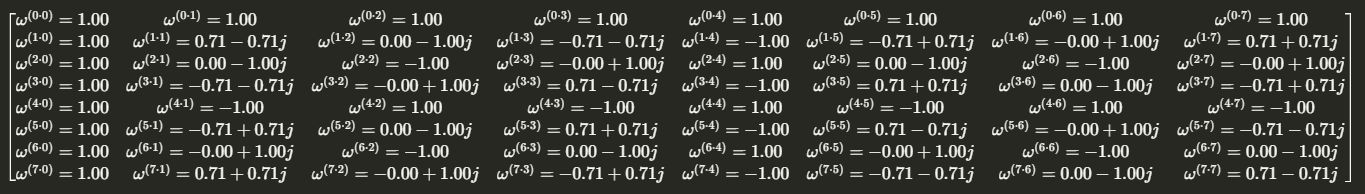
\includegraphics[width=1.2\textwidth]{fig5.png}
    \caption{Matricea Fourier 8x8}
    \label{fig:fig5}
\end{figure}

\begin{minted} {python}
fig, axs = plt.subplots(N, 3, figsize=(15, 16)) # 8 linii, 3 coloane
for i in range(N):
    axs[i, 0].set_ylabel(f"linia {i}")
    axs[i, 0].plot(F[i].real, label='real', color='green')
    axs[i, 0].plot(F[i].imag, label='imaginar', color='orange')
    axs[i, 0].stem(F[i].real)
    axs[i, 0].stem(F[i].imag)
    #axs[i, 0].legend()
    axs[i, 1].plot(F[i].real, color='green')
    axs[i, 1].set_title("partea reala")
    axs[i, 2].plot(F[i].imag, color='orange')
    axs[i, 2].set_title("partea imaginara")

plt.tight_layout()
plt.show()
\end{minted}

\begin{figure}[H]
    \centering
    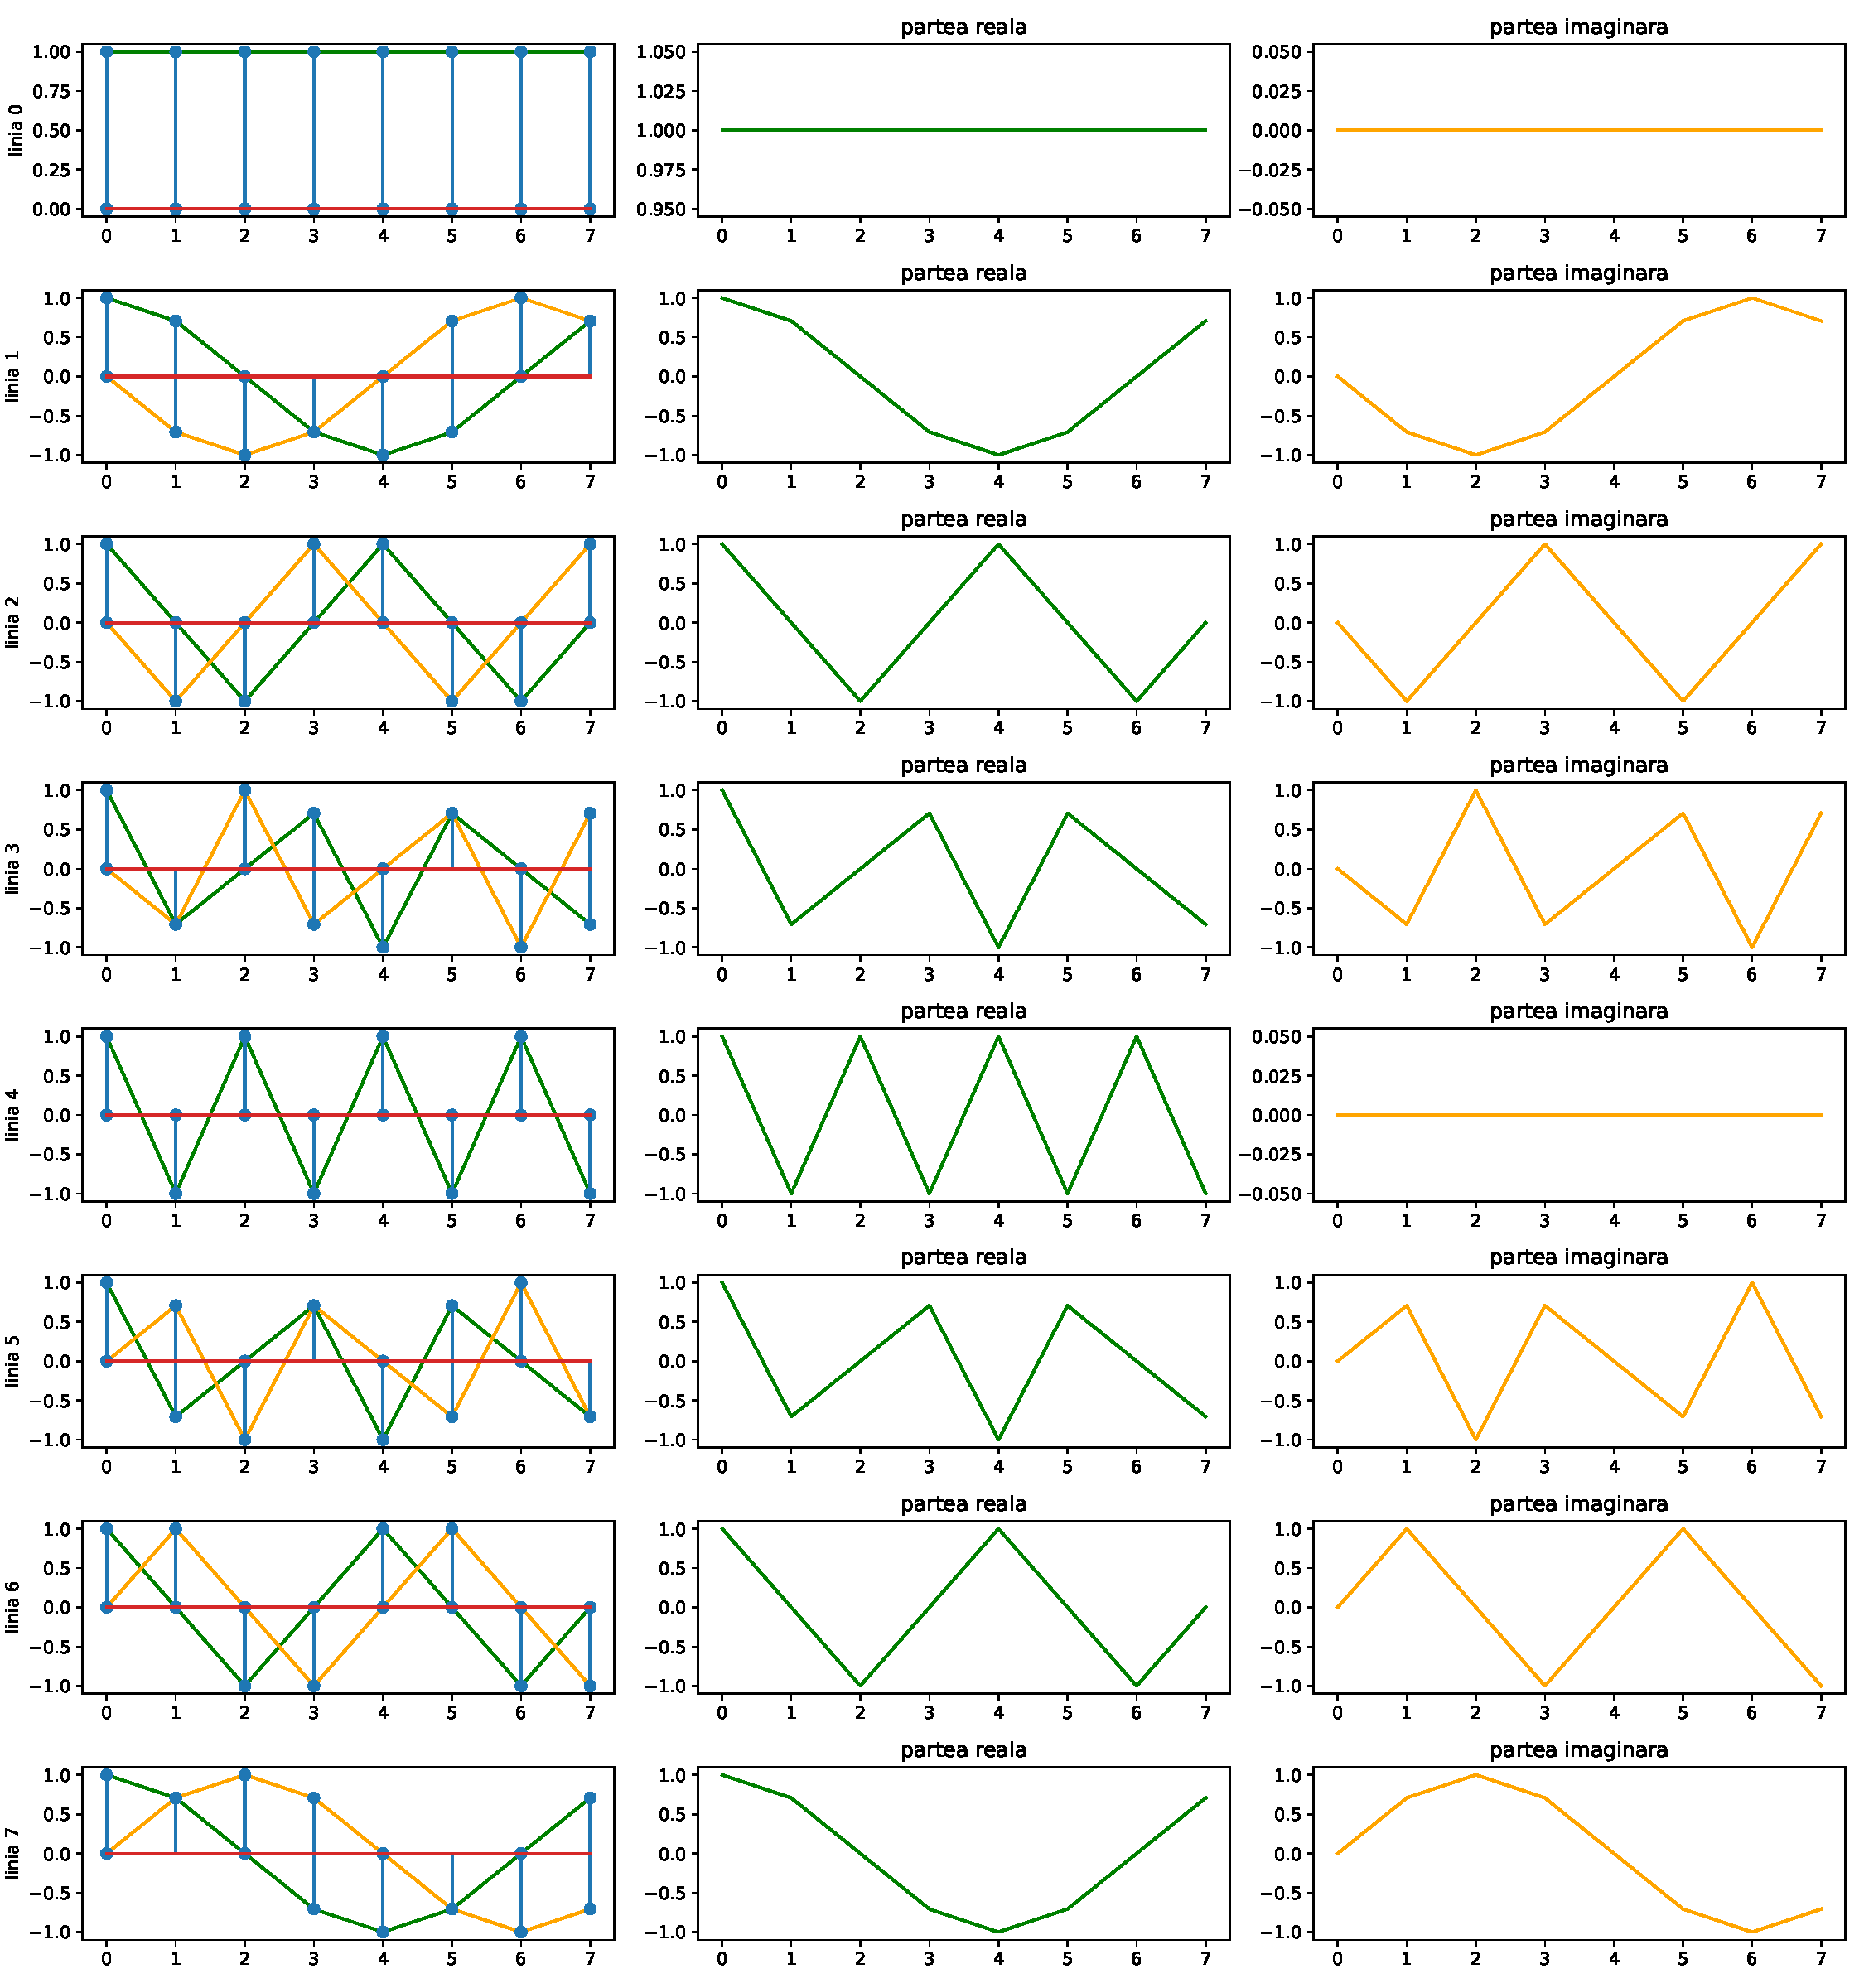
\includegraphics[width=1.2\textwidth]{fig6.pdf}
    \caption{Partea reală și imaginară}
    \label{fig:fig6}
\end{figure}

\section*{Bibliografie}
\begin{itemize}
\item \url https://www.statlect.com/matrix-algebra/discrete-Fourier-transform
\item \url https://erickson.academic.wlu.edu/files/courses2020/sigproc_s2020/readings/DFT_Intro.pdf 
\item \url https://www.robots.ox.ac.uk/~sjrob/Teaching/SP/l7.pdf
\item \url https://visionbook.mit.edu/image_processing_fourier.html
\item \url https://math.fandom.com/ro/wiki/Serie_Fourier

\end{itemize}
\end{document}
